% !TeX root = RJwrapper.tex
\title{Music Data Analysis in \texttt{R} - Short course, \\
Technical report}
\author{by Bruna Wundervald}

\maketitle

\abstract{
Music Information Retrieval (MIR) is a recent study field, with
a wide range of applications yet to be explored. It combines
computational tools with music theory to amplify the utility
of music data of many different formats. Each data format
carries dissimilar levels of information,  represented
as sheet music, audio files, chords, lyrics, and others. On the
Music Data Analysis in \texttt{R} short course, we presented
some possible applications of MIR using \texttt{R}, including:
i) accessing data from APIs; 
ii) sentiment analysis in music lyrics; iii) harmony analysis; 
iv) visualization, and v) music popularity prediction with machine
learning models. All applications made direct use of 
\texttt{R}, including especially the \texttt{tidyverse}, 
\texttt{vagalumeR}, \texttt{RSpotify} and \texttt{chorrrds} 
package. 
}


\section{Introduction}

On May 21 to 23, 2019, the IV International Seminar on 
Statistics with \texttt{R} took place in Niter\'oi, Brazil, 
with the theme 'R & Python collaboration trends'. 
As a part of the event, there was also a short-course day,
on May 20, when the Music Data Analysis in \texttt{R} (\cite{musicdatainR}) was presented. 

Music Information Retrieval (MIR) is a recent study field, with
a wide range of applications yet to be explored. It combines
computational tools with music theory to amplify the utility
of music data of many different formats. Each data format
carries dissimilar levels of information, being represented
as sheet music, audio files, chords, lyrics, and others.

Since Music Information Retrieval is still mostly done
in \texttt{python}, it made sense to bring this short-course
to such an event. The main idea of the course is to show
how MIR can be done in \texttt{R} (\cite{R}), and still has a lot
of space to grow inside the community. We presented
some possible applications of MIR using \texttt{R}, including:
i) accessing data from APIs; 
ii) sentiment analysis in music lyrics; iii) harmony analysis; 
iv) visualization;  and 
v) music popularity prediction with machine learning models. 

\section{Audience}

This short-course was meant to be for anyone interested in 
\texttt{R} or music information retrieval. The final audience 
consisted mainly of students with an intermediate level of
\texttt{R} and data analysis. 

\section{Description}

All applications of the short-course made direct use of 
\texttt{R}. For this course, we choose to work with the data of the Brazilain singer Chico Buarque, to demonstrate the 
content of the course. The main goals of the material 
presented were, first, to show how to use the packages:

\begin{itemize}
    \item \texttt{vagalumeR}: lyrics extraction
    \item \texttt{chorrrds}: chords extraction
    \item \texttt{Rspotify}: extract variables from the Spotify API
\end{itemize}

All the 3 packages were used for the data extraction. 
As the \texttt{vagalumeR} and \texttt{Rspotify} makes use of 
2 different APIs, the short-course also covered an introduction
about how to connect and handle the access to APIs in 
\texttt{R}. 

With the data in hand, the next task was to learn how to 
combine data from different sources. The main issue, in this
case, was that, in theory, it exists a common key between
the 3 data sources, which is the song names, 
but that might not always be true. Sometimes, the names
are written slightly different, or even completely, and this needs
to be addressed properly when we are treating the data.

We followed into the understanding and summarising of the 
obtained data, which comes in various formats:
\begin{itemize}
    \item Text,
    \item Continuous variables,
    \item Sequences.
\end{itemize}


For the text data, the lyrics, we focused on visualization,
tokenization, sentiment analysis, leading us to find interesting
features such as the most common words and bi-grams and in which songs the most positive or negative feelings are.  

For the chords data, on the other hand, we had a bit
more of work related to music theory. We found which
were the songs more harmonically "complex", as in evaluating
their harmonic structures, number of distinct chords and
by extracting harmonic variables. We do the last one 
because the chords, in reality, are nothing but a string, 
which does not mean anything quantitatively. Because of 
this, feature extraction is necessary if we want to make
more sense of it. Besides that, we also evaluated the
most common or rare chords transitions, seeing how it agreed
with music theory rules, that define which transitions 
make more sense. 

Next, we used the variables from the Spotify API 
to discover how the popularity of the songs varies in the
dataset, what are the least and most popular songs and
a little of exploratory analysis, to check what is the relationship between the danceability and the other variables originated in the API. This leads us to the final
part of the course, which consisted of the creation
of prediction models for the popularity of the songs. In 
this case, we decided to use the random forest model
(\cite{Breiman2001}), 
and the variables that were obtained throughout the course. 


The short-course was presented with the help of slides 
and the RStudio IDE, where the code in the presentation
was run. It was originally presented in Portuguese, 
but an English version of all the material was also made
publicly available. The slides in both languages, as
well as the data and the code (\texttt{.R} file),  are
hosted at \texttt{https://github.com/brunaw/SER2019}.


\section{Course evaluation}

In the end, it was asked for the students to fill
a quick evaluation form. Not all students answered, 
and the results are presented in Figure 1. 
There is quite a good appreciation for the material and 
the presentation of the short-course, demonstrating the
need for \texttt{R} material in the area. 
Even with that, the students considered the class a little faster than the ideal, meaning that it could 
have had a better pace. The content has split the opinions, 
being considered perfect for a few students, but a little
hard for some others. 


\begin{figure}[ht]
  \centering
  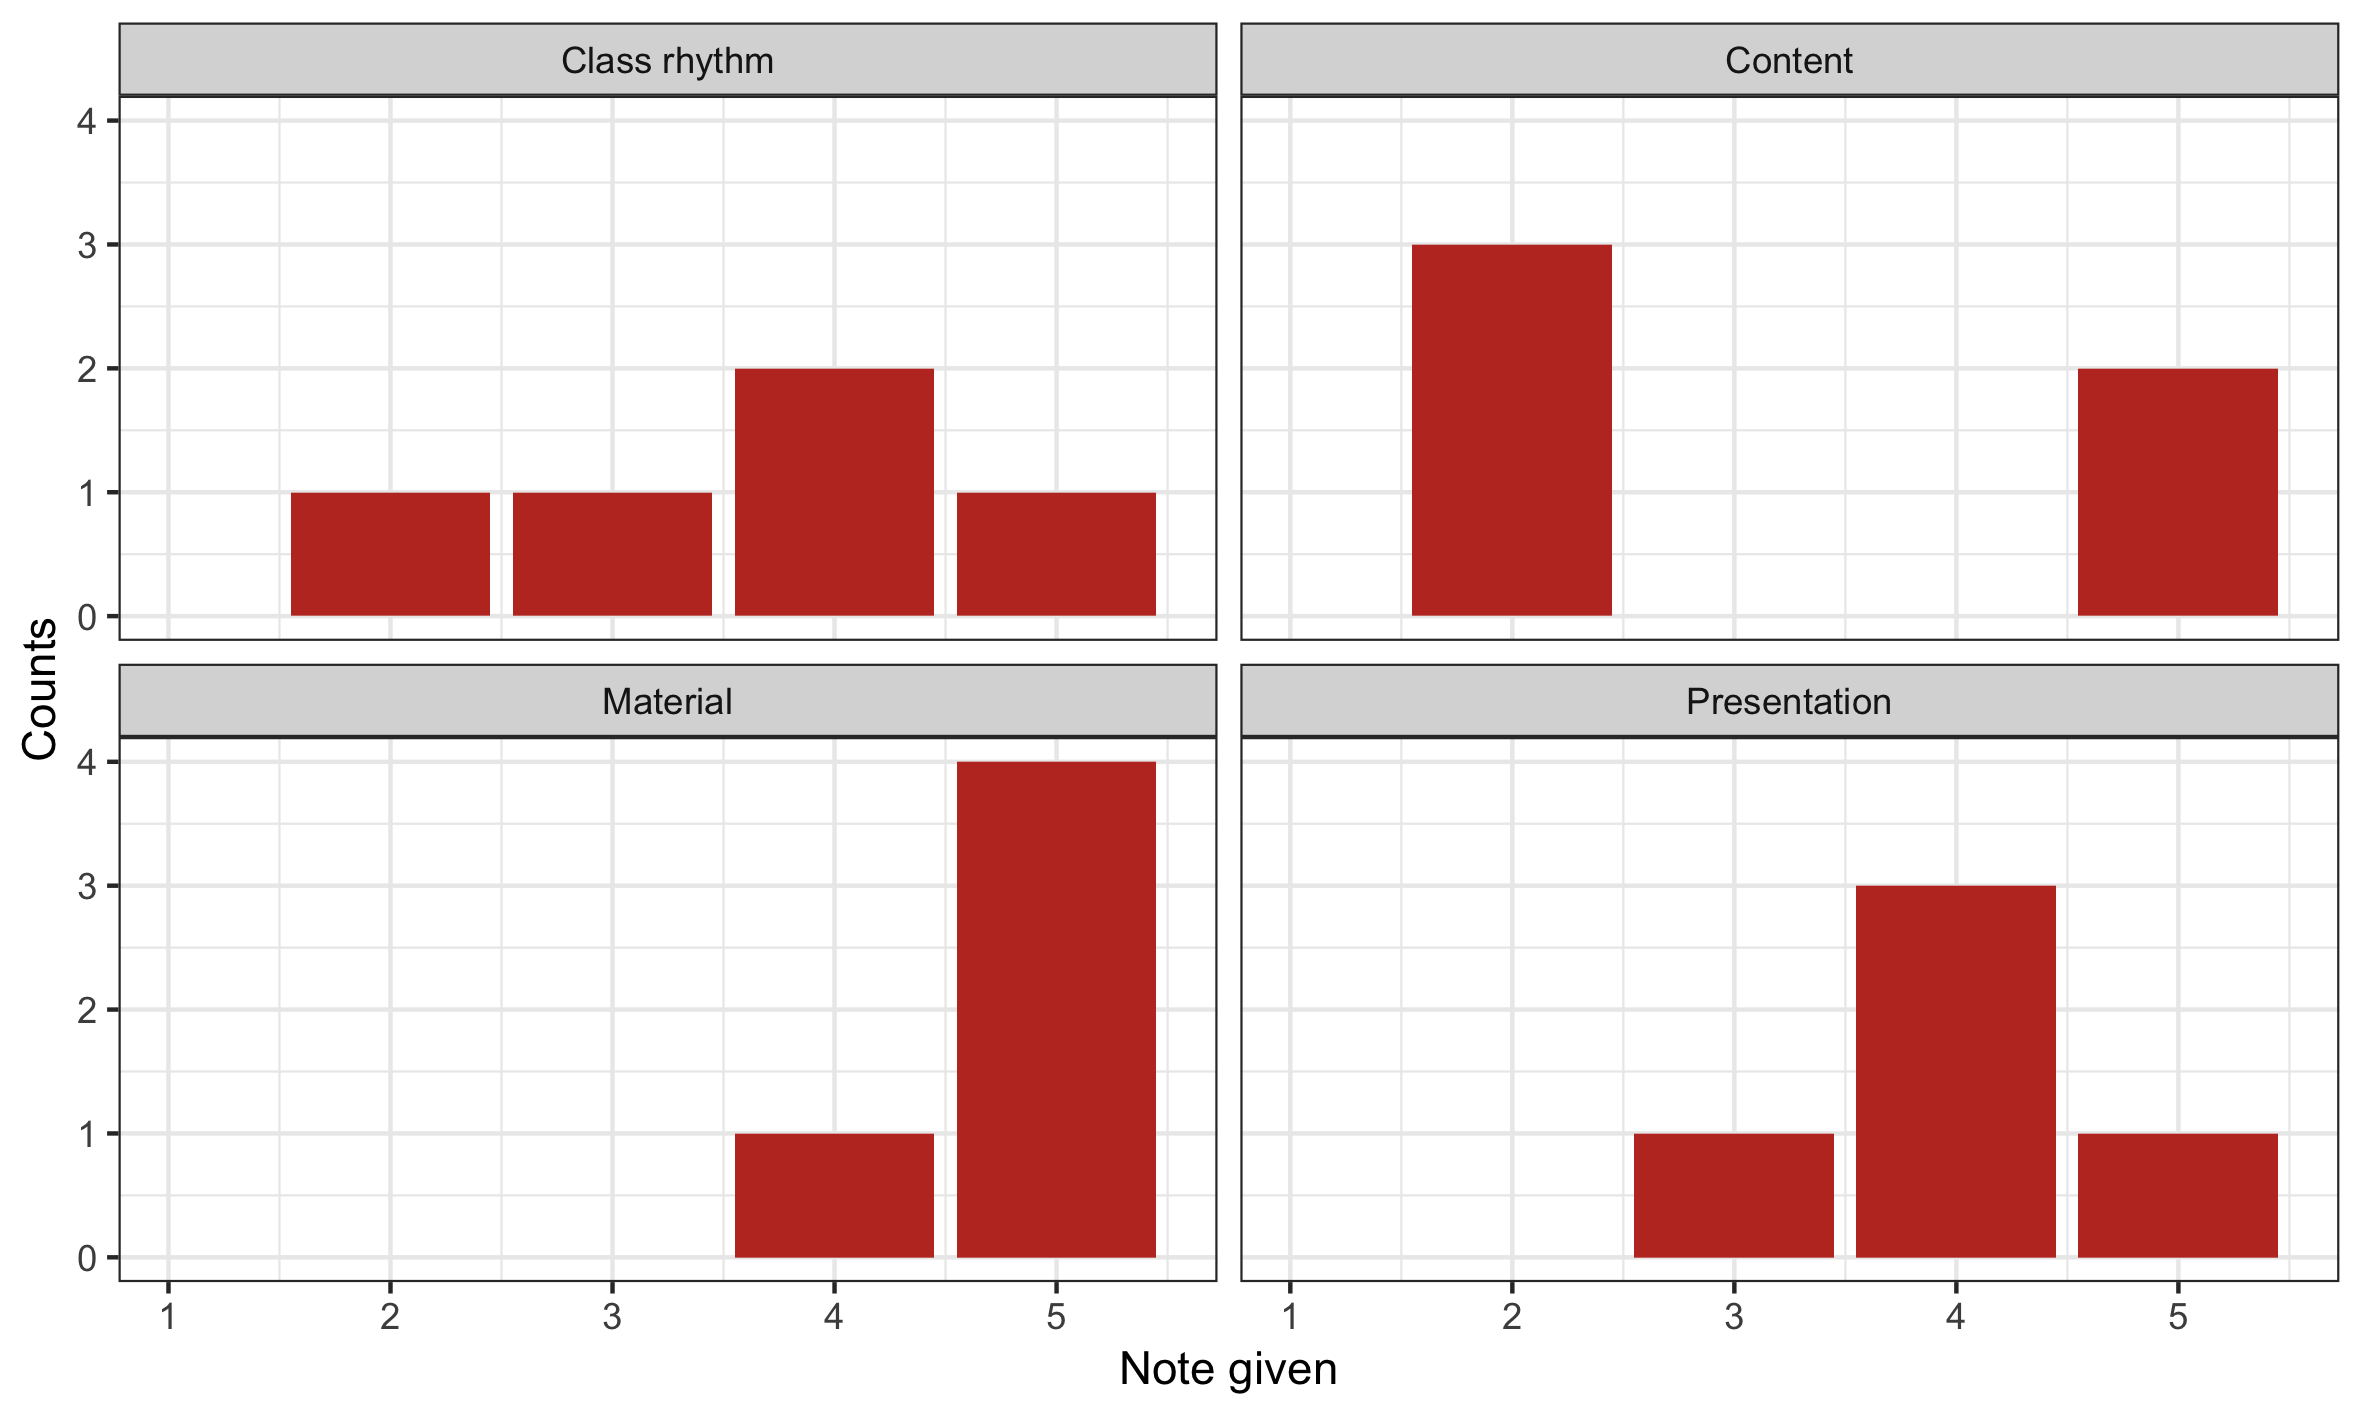
\includegraphics[width=13cm, heigth=22cm]{results.png}
  \caption{Final evaluation of shortcourse. 3 represents perfect for the Class rhythm, and 5 represents perfect for the other questions. }
  \label{figure:rlogo}
\end{figure}


\section{Next steps}

Some reviews about this course are planned, 
in order to make it clearer/accessible to more people. 
We would like to produce more material about 
\texttt{R} regarding music data 
analysis, as this increase of availability 
can help strengthen such a young community and
the Music Information Retrieval area in general. 




\bibliography{references}

\address{Bruna Wundervald\\
  Maynooth University, Maynooth, Ireland\\
  \email{brunadaviesw@gmail.com}}

